% -*- root: ../main.tex -*-
%!TEX root = ../main.tex
% this file is called up by main.tex
% content in this file will be fed into the main document
% vim:textwidth=80 fo=cqt

\graphicspath{{4/figures/}}
% ----------------------- contents from here ------------------------

\chapter{Computational Analysis and Numerical Reformulation of the \glsfmtshort{dra}}\label{ch:improveddra}
% \chapter{Analysis of the \glsfmtlong{dra} and Performance Boost through Numerical Reformulation}\label{ch:improveddra}
% \chapter{Computational Bottleneck Analysis of the \glsfmtshort{dra} and its Mitigation through Numerical Reformulations}\label{ch:improveddra}
\startcontents[chapters]
\printcontents[chapters]{}{1}{\setcounter{tocdepth}{1}}

\bigskip

\capolettera{T}{his} chapter presents  an analysis and critical  evaluation of a
computational bottleneck present  in a popular \gls{rom}  framework and proposes
an  alternative numerical  reformulation  to  mitigate it\footnote{This  chapter
is  based  on the  journal  publication  --- \fullcite{Gopalakrishnan2017}.  All
intellectual ideas in  the aforementioned article are  original contributions of
this  thesis  author.  All  text,  tables, figures  and  captions  therein  were
contributed solely by this thesis author. Copyright clearance for non-commercial
verbatim  reproduction  of  the  content  (such as  in  this  thesis)  has  been
secured  through  the  publication  agreement with  the  copyright  holder  ASME
(see~\cref{ch:permissions}). The contents in this chapter  may be, in full or in
part,  included  verbatim from  the  said  publication.  This author  wishes  to
express  his  thankfulness  to  Teng  Zhang,  co-author  of  this  article,  for
checking my calculations  and providing valuable feedback that  helped to refine
the  manuscript  for that  journal  publication.}.  From the  literature  review
presented  in~\cref{ch:littreview},  it  may  be  recalled  that  transcendental
transfer  functions  of  the  cell's  electrochemical  field  variables  (except
for  concentration   and  potential   in  the   electrolyte)  was   obtained  by
Smith~\etal~\cite{Smith2007} through  linearisation of the  underlying \gls{p2d}
model  equations. Lee~\etal~\cite{Lee2012a,Lee2012}  extended  this approach  to
obtain  the  missing  electrolyte   transfer  functions  through  a  multi-modal
EigenFunction expansion employing a Sturm-Liouville approach~\cite{Pryce1993}.


In  order  to  obtain  a  \gls{lti} state-space  representation  of  the  system
(see~\cref{eq:LTIstatespace}) for  embedded implementation,  Lee~\etal{} devised
the   \gls{dra},  a   numerical  procedure   to  systematically   transform  all
transcendental  transfer functions  to  the time  domain.  The \gls{dra}  method
retains  the physical  nature  of  the original  \gls{dfn}  equations until  the
very  last  step  wherein  the  matrices governing  the  system's  dynamics  are
generated. This  yields a  one-dimensional discrete-time  \gls{rom} of  the cell
that is entirely based upon  fundamental physical principles. The \gls{rom} thus
obtained could  then be used to  compute the time-evolution of  all the internal
electrochemical quantities of  the \gls{dfn} model. Prima~facie  it appears that
this  model  could be  directly  implemented  as the  plant  model  for a  state
estimation  application.  However, a  comprehensive  analysis  of the  procedure
reveals  a critical  issue  that  must be  first  tackled before  implementation
aspects can be considered.

The unresolved  issue in  Lee's approach is  the excessively  high computational
requirements associated  with the  \gls{dra}, which  becomes a  bottleneck since
it  needs  to  be  repeated  for multiple  \glspl{soc}  and  temperatures.  This
computational  bottleneck  arises  from  forming  a  large  Block-Hankel  matrix
in  memory  upon  which  a  \gls{svd} is  performed.  Under  certain  conditions
as  discussed  in~\cref{subsec:Size-of-the}, owing  to  the  large size  of  the
Block-Hankel  matrix, the  \gls{dra} computation  is rendered  intractable. This
issue  has been  acknowledged by  the authors~\cite{Lee2012,Plett2015}.  In this
chapter, this  computational bottleneck  is analysed and  an improved  scheme is
proposed.  \Cref{sec:Analysis-of-the}  discusses  an  analytical  evaluation  of
the  massive  computing requirements  of  Lee's  \gls{dra} method.  Redundancies
and  inefficiencies in  this  step  are enumerated  and  the high  computational
costs are deemed as  unnecessary. In~\cref{sec:Efficient-Computation-of}, a fast
computational  approach  is  presented  which  significantly  reduces  both  the
memory  and computational  time  of the  \gls{rom} workflow.  \Cref{sec:Results}
summarizes  the   results  obtained  from  applying   the  algorithms  discussed
in~\cref{sec:Efficient-Computation-of}  by comparing  and  contrasting the  much
smaller computational requirements of the new method with the existing \gls{dra}
scheme.  Furthermore,  improved modelling  accuracy  achieved  by this  proposed
method,  when deployed  under  resource-constrained  computing environments,  is
highlighted.  \Cref{sec:Conclusion}  concludes  the  chapter with  a  view  that
although the improved  methodology streamlines the entire  workflow, there exist
some fundamental deficiencies in Lee's hybrid modelling approach that impede its
effective deployment as the plant model in state-estimation tasks.

\section{Analysis of the Computational Bottlenecks of the \glsfmtshort{dra}} \label{sec:Analysis-of-the}

The \gls{rom}  proposed by  Lee~\etal{} aims  for the  simplified representation
of  the  \glsfirst{p2d}  volume-averaged  continuum  model  proposed  by  Doyle,
Fuller   and   Newman~\cite{Doyle1993a,Fuller1994}\footnote{hereafter   referred
interchangeably in  this thesis  by the two  acronyms ---  \glsfmtshort{dfn} and
\glsfmtshort{p2d}.}.


The  block diagram  in~\cref{fig:traditional_ROM_Workflow}  depicts the  overall
modelling workflow. First,  the governing PDE equations are  linearised about an
operating point  of \gls{soc} and temperature.  Then, closed-form Laplace-domain
transcendental  transfer  functions  of  all the  internal  physical  quantities
$\left(\phi_{s},\phi_{e},c_{s},c_{e},j\right)$  at   different  cell  locations,
are  derived  using applied  current  as  the  input.  A detailed  treatment  of
the  analytical  derivation  is   presented  in  Lee~\etal~\cite{Lee2012a}.  The
authors  proposed  a novel  \glsfirst{dra}  scheme~\cite{Lee2012b}  in order  to
transform  these  transcendental  transfer  functions  to  standard  state-space
representation.   Sublevel-1   of~\cref{fig:traditional_ROM_Workflow}  shows   a
breakout view of  the \gls{dra} procedure and illustrates the  steps involved in
this  computation. At  the  heart  of this  numerical  method  is the  classical
subspace  identification approach  known as  Ho-Kalman algorithm~\cite{HO1966a},
whose  computation  steps  are  shown   via  the  exploded  view  in  sublevel-2
of~\cref{fig:traditional_ROM_Workflow}. Markov  parameters (unit-pulse response)
of this \gls{simo} linear system of battery transfer functions is computed. They
form the entries  of a Block-Hankel matrix~\cite{Ljung1998},  wherein each block
element is a column vector of the set of Markov parameters at a given time-step.
A  key computation  in the  Ho-Kalman algorithm  is the  \glsfirst{svd} of  this
Block-Hankel  matrix. A  wide separation  in magnitude  drop between  successive
singular values serves as a guide in choosing the desired \gls{rom} order.

\begin{figure}[!htbp]
    \centering
    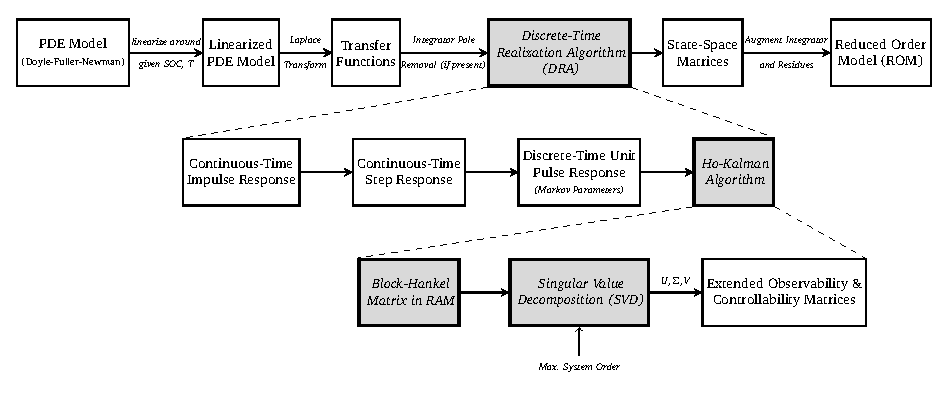
\includegraphics[width=\textwidth]{traditional_dra.eps}
    \caption[%
    Reduced-order modelling (ROM) workflow using classical \glsfmtshort{dra}.
    ]%
    {%
        Reduced-order modelling (ROM) workflow using classical
        \glsfmtshort{dra}. The shaded blocks represent computational bottlenecks.
    }%
    \label{fig:traditional_ROM_Workflow}
\end{figure}

The    analyses     presented    in~\cref{subsec:Traditional-DRA--Memory}    and
\cref{subsec:Traditional-DRA--CPU}  reveal  major  inefficiencies  in  both  the
Block-Hankel  formation and  the \gls{svd}  computation steps  which hinder  the
entire reduced-order modelling workflow.

\subsection{Classical \glsfmtshort{dra} --- Memory (\glsfmtshort{ram}) Requirements}\label{subsec:Traditional-DRA--Memory}

% Lee et al.~\citep{LeeChemistruckPlett2012} modeled 28 transfer functions,
% representing electrochemical variables at the current collector and
% separator interfaces. Each Markov parameter is a 28 element column
% vector. 16000 time-samples was obtained at a sample-rate of 1 Hz,
% allowing sufficient time for the Markov parameters of the slowest
% dynamics, i.e. solid surface concentration to settle to an acceptably
% low magnitude. The Block-Hankel matrix thus formed has 8000 blocks,
% each block consisting of 28 elements. The Block-Hankel matrix thus
% has $8000\text{ x }28=224000$ rows and 8000 columns. Hence, the overall
% number of elements in the Block Hankel matrix is $224000\text{ x }8000=1.79\text{ x }10^{9}$.
% Using double-precision arithmetic, its storage requirement can be
% estimated to be approximately 27 GB.

% Computing the SVD results in formation of three more large matrices
% in memory \textendash{} matrix of output singular vectors $\left(U\right)$,
% matrix of input singular vectors $\left(V\right)$ and the diagonal
% singular-value matrix $\left(\Sigma\right)$. With 8000 Hankel-blocks,
% approximately 81 GB of RAM is required for holding these three output
% matrices generated by a full-SVD. However, the intermediate operational
% memory usage during the SVD computation is often much higher than
% the combined size of all the matrices. As these large matrices must
% be handled at each operating point of SoC and temperature, the high
% memory demand of classical DRA remains a persistent issue.


\subsection{Classical \glsfmtshort{dra} --- \glsfmtshort{cpu} Operation Count}\label{subsec:Traditional-DRA--CPU}

% The most widely used numerical algorithm for computing the full SVD
% of a generic dense matrix $\mbox{\ensuremath{A\in\mathcal{R}^{mxn},m\geq n}}$
% is the two-stage Golub-Kahan-Reinsch method~\citep{GolubVanLoan2012}.
% In the first stage $A\in\mathcal{R}^{mxn}$ is reduced to an upper
% bidiagonal form. In the second stage, SVD of this upper bidiagonal
% matrix, $B\in\mathcal{R}^{mxn}$ is computed using an iterative procedure
% such as the Demmel-Kahan method~\citep{GolubVanLoan2012}. If stage
% I of the SVD computation employs $\mathcal{R}$~-~Bidiagonalization~\citep{GolubVanLoan2012},
% then the overall process is referred to as $\mathcal{R}$\textminus SVD.
% This is the fastest known full-SVD computation method that may be
% applied to this battery modeling problem. The \textsc{DGESVD} algorithm~\citep{AndersonBaiBischofEtAl2012},
% originally implemented in LAPACK, employs this method. This has been
% ported to many numerical computation packages such as MATLAB, GNU
% Octave and Scilab. Several numerical libraries such as NAG and Intel
% MKL also use the DGESVD codes due to its acclaimed stability, robustness
% and versatility. The MATLAB implementation \texttt{\textbf{svd}} is
% also based upon DGESVD, and hence this can be considered as the de-facto
% baseline SVD code.

% The operation count for computing the singular values and vectors
% of a generic dense matrix $\mbox{\ensuremath{A\in\mathcal{R}^{mxn},m\geq n}}$
% using the $\mathcal{R}$\textminus SVD method is $\mbox{\ensuremath{4m^{2}n+22n^{3}}}$~\citep{GolubVanLoan2012}.
% Markov parameters of $x$~transfer functions and $N$ time-samples
% yields a Block-Hankel matrix with $m=xN$ rows and $n=N$ columns.
% Hence,
% \begin{alignat}{2}
% CPU\text{ Operation Count} & = & \,4\left(xN\right){}^{2}N+22N^{3}\nonumber \\
% & = & \,2N^{3}\left(11+2x^{2}\right)\label{eq:cpu_op_count}
% \end{alignat}
% Thus the CPU operation count scales as $\mathcal{O}(N^{3})$
% with the number of Markov time-samples$\left(N\right)$ and as $\mathcal{O}(x^{2})$
% with the number of transfer functions being modeled. The ROM computed
% in Lee et al. uses 28 transfer functions wherein the Markov parameters
% are collected for 16000 seconds with a sampling interval of 1 second.
% Thus, the CPU operation count for performing this computation is approximately
% $\mathcal{O}(16000^{3})\sim4\text{ x }10^{12}$ floating point operations
% (\textit{flops}).


\subsection{Size of the Block-Hankel Matrix\label{subsec:Size-of-the}}

% Large Block-Hankel matrices can occur in DRA computation due to the
% following reasons.
% \begin{enumerate}
% 	\item For a given duration of Markov-parameter recording, if a high sample-rate
% 	ROM is desired, the emulation frequency has to be proportionately
% 	increased. This is for accurately computing the continuous-time step
% 	and pulse responses in Figure~\ref{traditional_ROM_Workflow}.
% 	This implies that the total number of time-samples $\left(N\right)$
% 	for each Markov parameter will have to be scaled proportionately to
% 	capture the desired duration of the unit-pulse-response. However,
% 	the size of the Block-Hankel matrix has a quadratic dependence on
% 	the Markov parameter length.
% 	\item The recorded sample size~$\left(N\right)$ could also become large
% 	if the Markov parameters of just one of the transfer functions decay
% 	very slowly. In Li-ion batteries, diffusion within the solid particle
% 	is typically the slowest process. For the cell modeled in Lee et al.,
% 	the unit-pulse response of surface concentration of Li adjacent to
% 	the positive current collector requires approximately 16000 samples
% 	before reducing to an appreciably low value, as shown in Figure~\ref{markov_cse_pos}.
% 	\item For a battery modeling problem consisting of multiple transfer functions,
% 	the number of entries in the Block-Hankel matrix also scales linearly
% 	with the number of transfer functions. Thus, if more cell variables
% 	(e.g. concentrations and potentials at other spatial locations within
% 	the cell) are to be studied, then the size of the transfer function
% 	vector and the Block-Hankel matrix increases correspondingly.
% \end{enumerate}
% Considering the combined influence of these effects, if $x$ transfer
% functions are to be modeled and $N$ time-samples of each Markov parameter
% are to be captured, the corresponding size of the Block-Hankel matrix,
% $H$ is
% \begin{equation}
% Size(H)\sim O(xN^{2})\text{ {entries}}\label{eq:}
% \end{equation}
% This has a significant computational impact as shown in Sections~\ref{subsec:Traditional-DRA--Memory}
% and \ref{subsec:Traditional-DRA--CPU}.
% \begin{figure}
% 	\caption{}
% 	\label{markov_cse_pos}
% \end{figure}

\section{Improved \glsfmtshort{dra} for Battery Modelling} \label{sec:Efficient-Computation-of}

